\section{Persistenz}
    \subsection{Classification Storage}
        Es wird eine Graphdatenbank verwendet!

    \subsection{Datenmodell}
        Wie sind die Daten in der DB modelliert?

        \begin{figure}
            \centering
            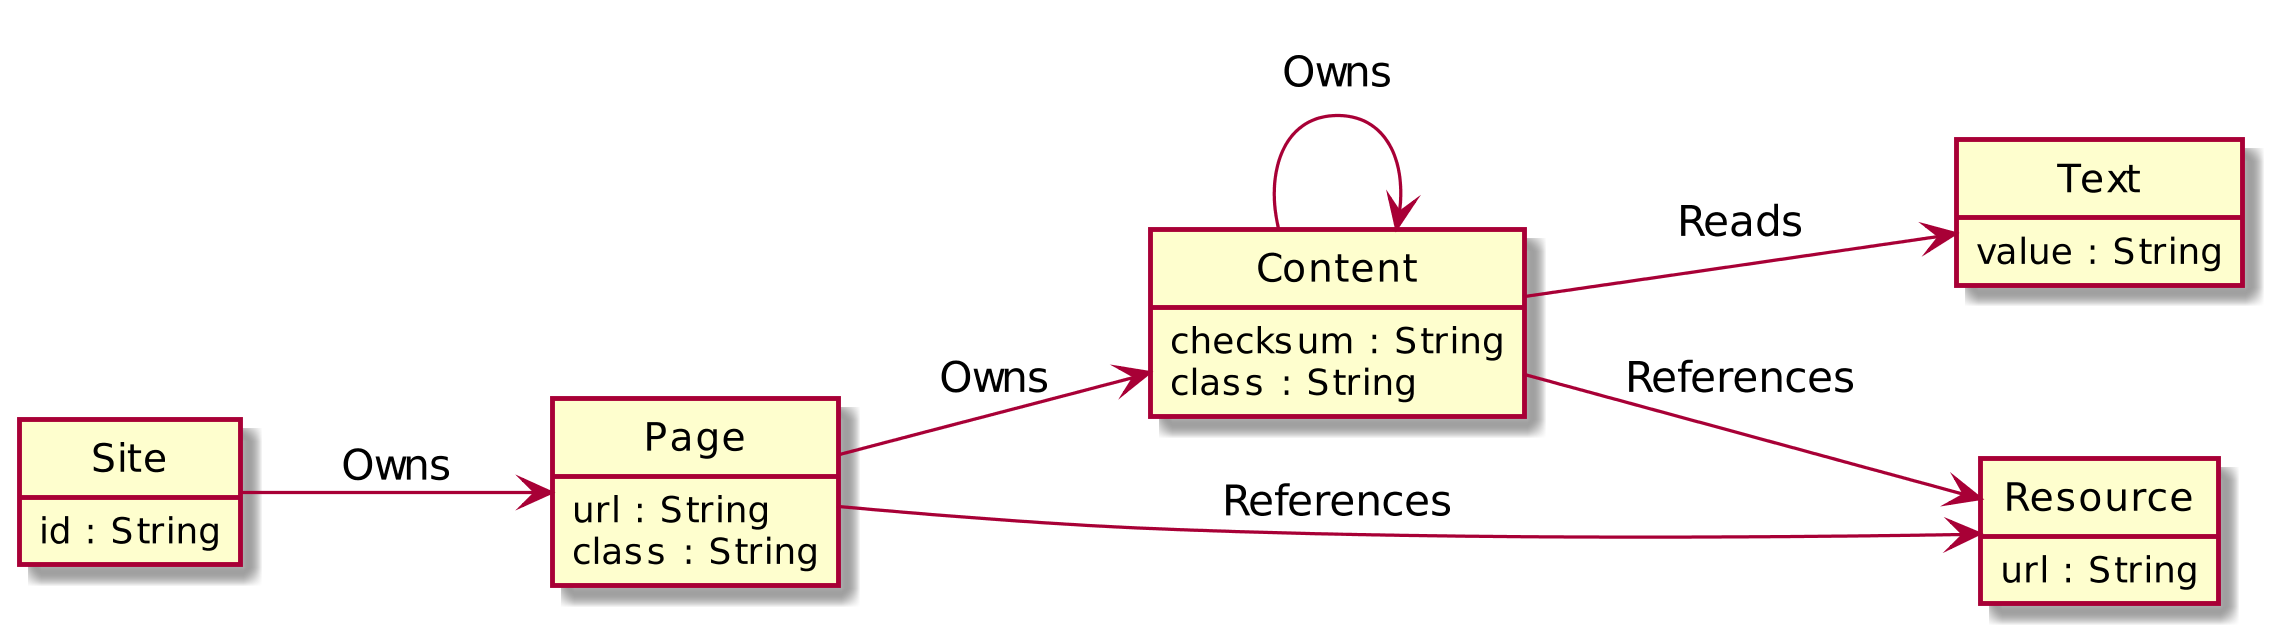
\includegraphics[width=\textwidth]{../resources/db-data-model/nodes.png}
            \caption{Übersicht der Nodes und ihrer Beziehungen}
            \label{image:dbDataModelOverview}
        \end{figure}

        \begin{figure}
            \centering
            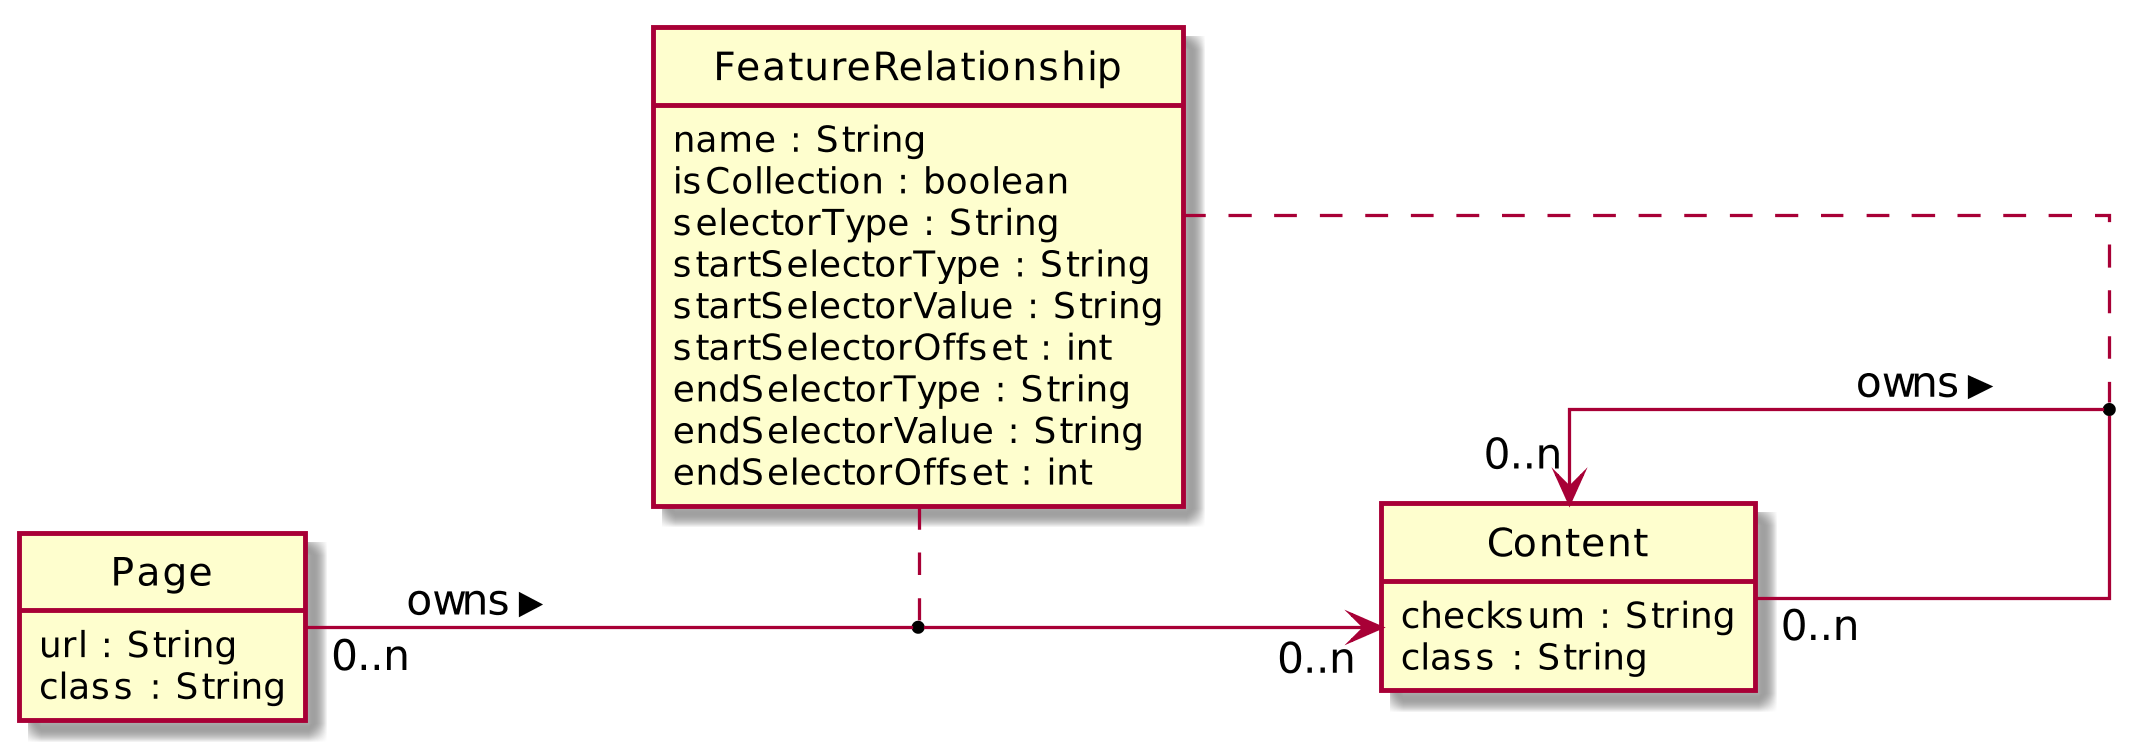
\includegraphics[width=\textwidth]{../resources/db-data-model/content-relationship.png}
            \caption{Content Features}
            \label{image:dbDataModelContentRelationship}
        \end{figure}

        \begin{figure}
            \centering
            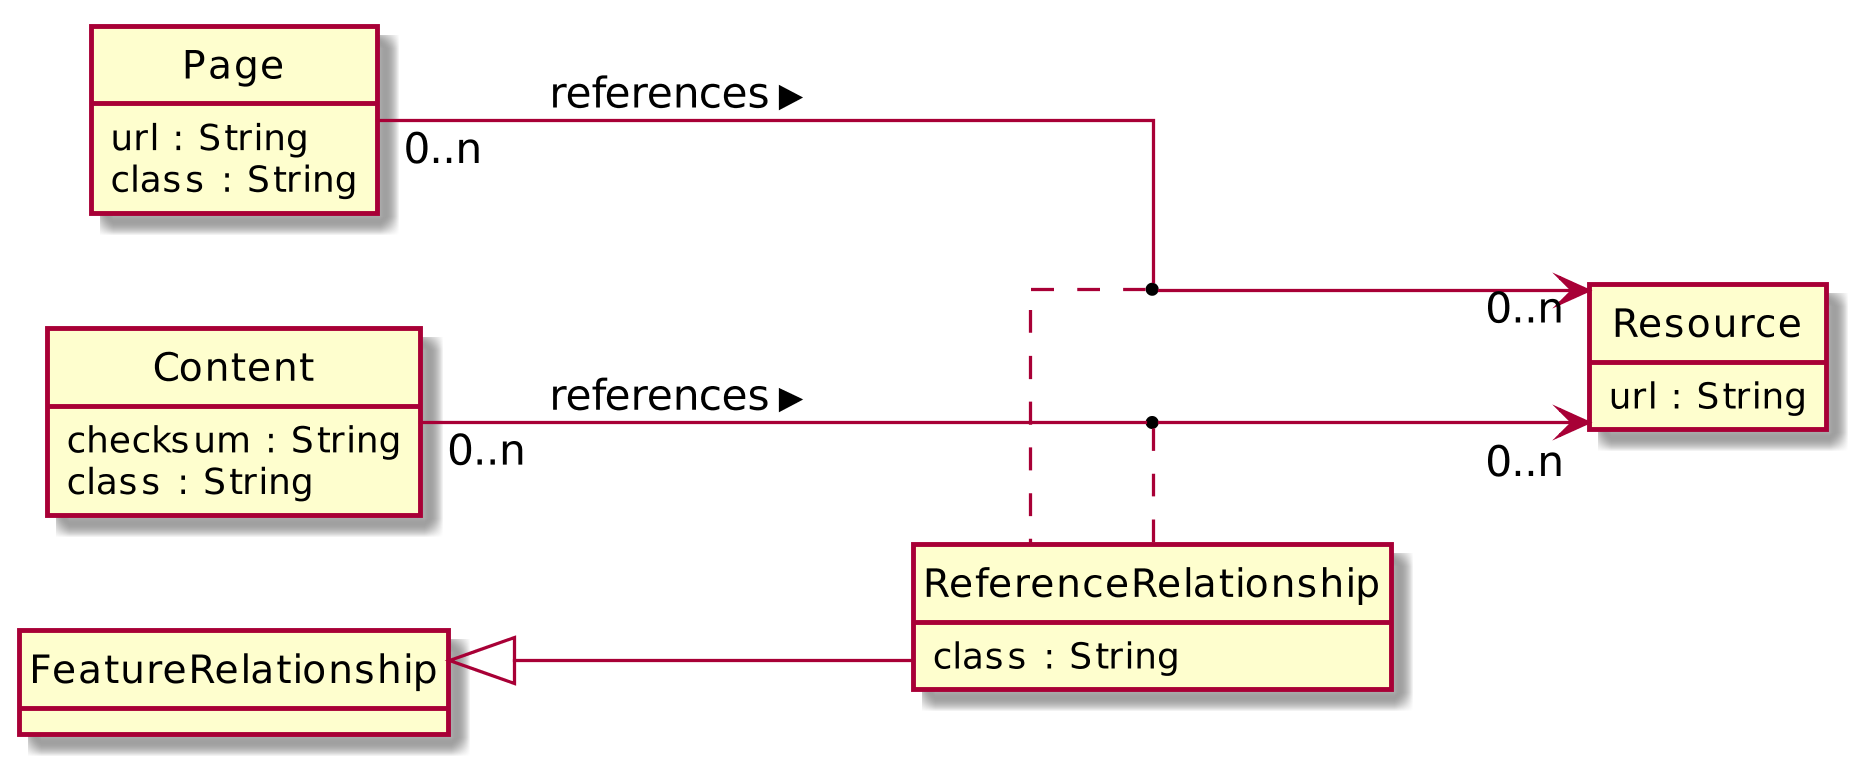
\includegraphics[width=\textwidth]{../resources/db-data-model/resource-relationship.png}
            \caption{Reference Features}
            \label{image:dbDataModelResourceRelationship}
        \end{figure}

    \subsection{Datenmodell Beispiel}
        \begin{figure}
            \centering
            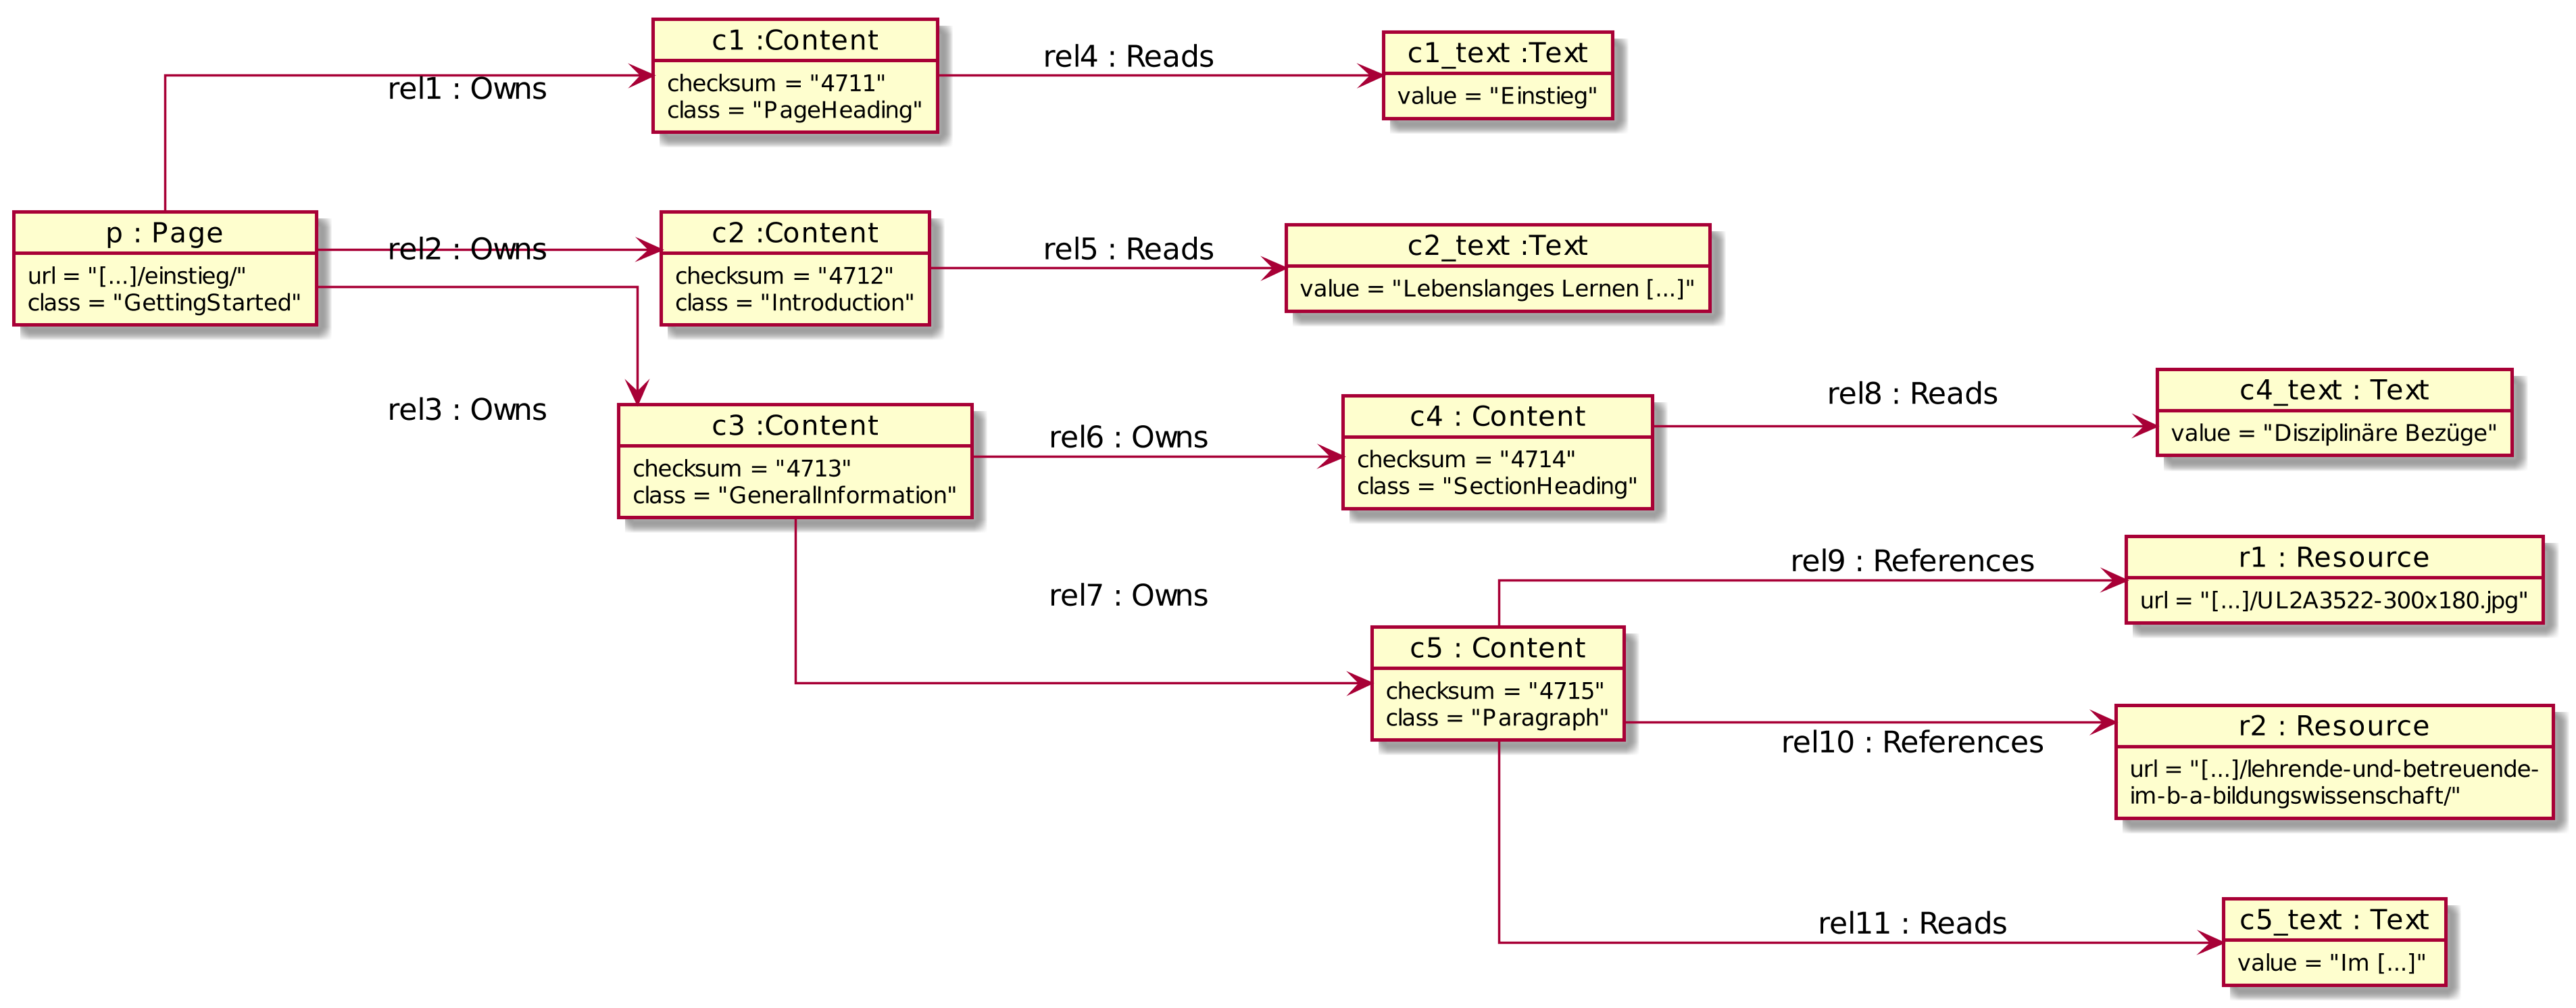
\includegraphics[width=\textwidth]{../resources/db-data-model/example/example.png}
            \caption{Beispiel}
            \label{image:dbDataModelExampleOverview}
        \end{figure}

        \begin{figure}
            \centering
            \begin{subfigure}{\textwidth}
                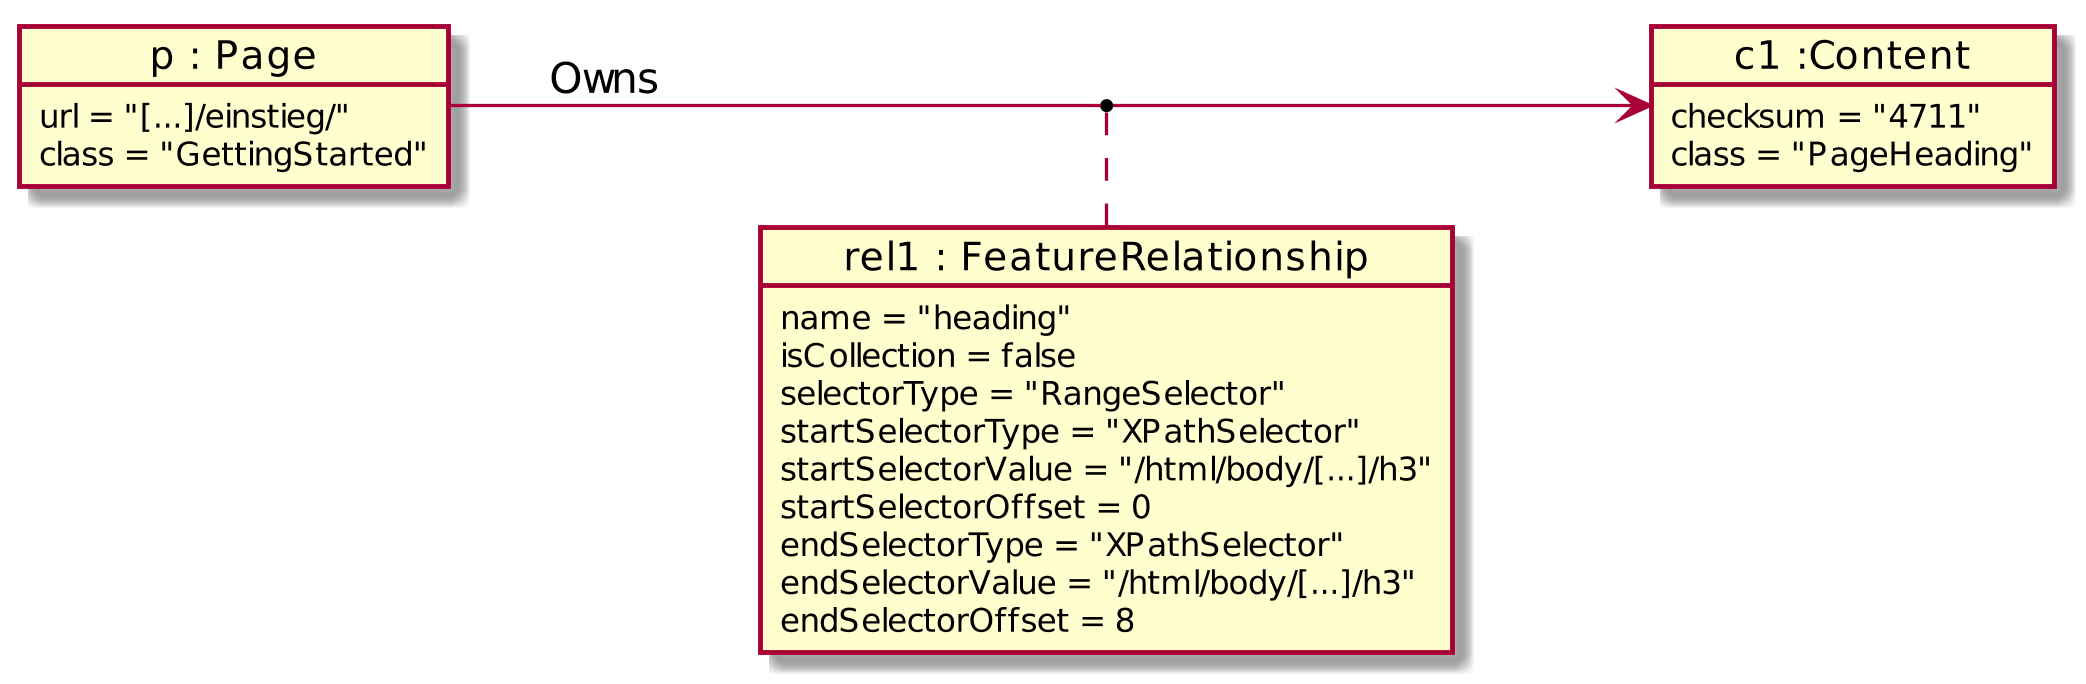
\includegraphics[width=\textwidth]{../resources/db-data-model/example/p-c1.png}
                \subcaption{Rel 1}                    
            \end{subfigure}

            \begin{subfigure}{\textwidth}
                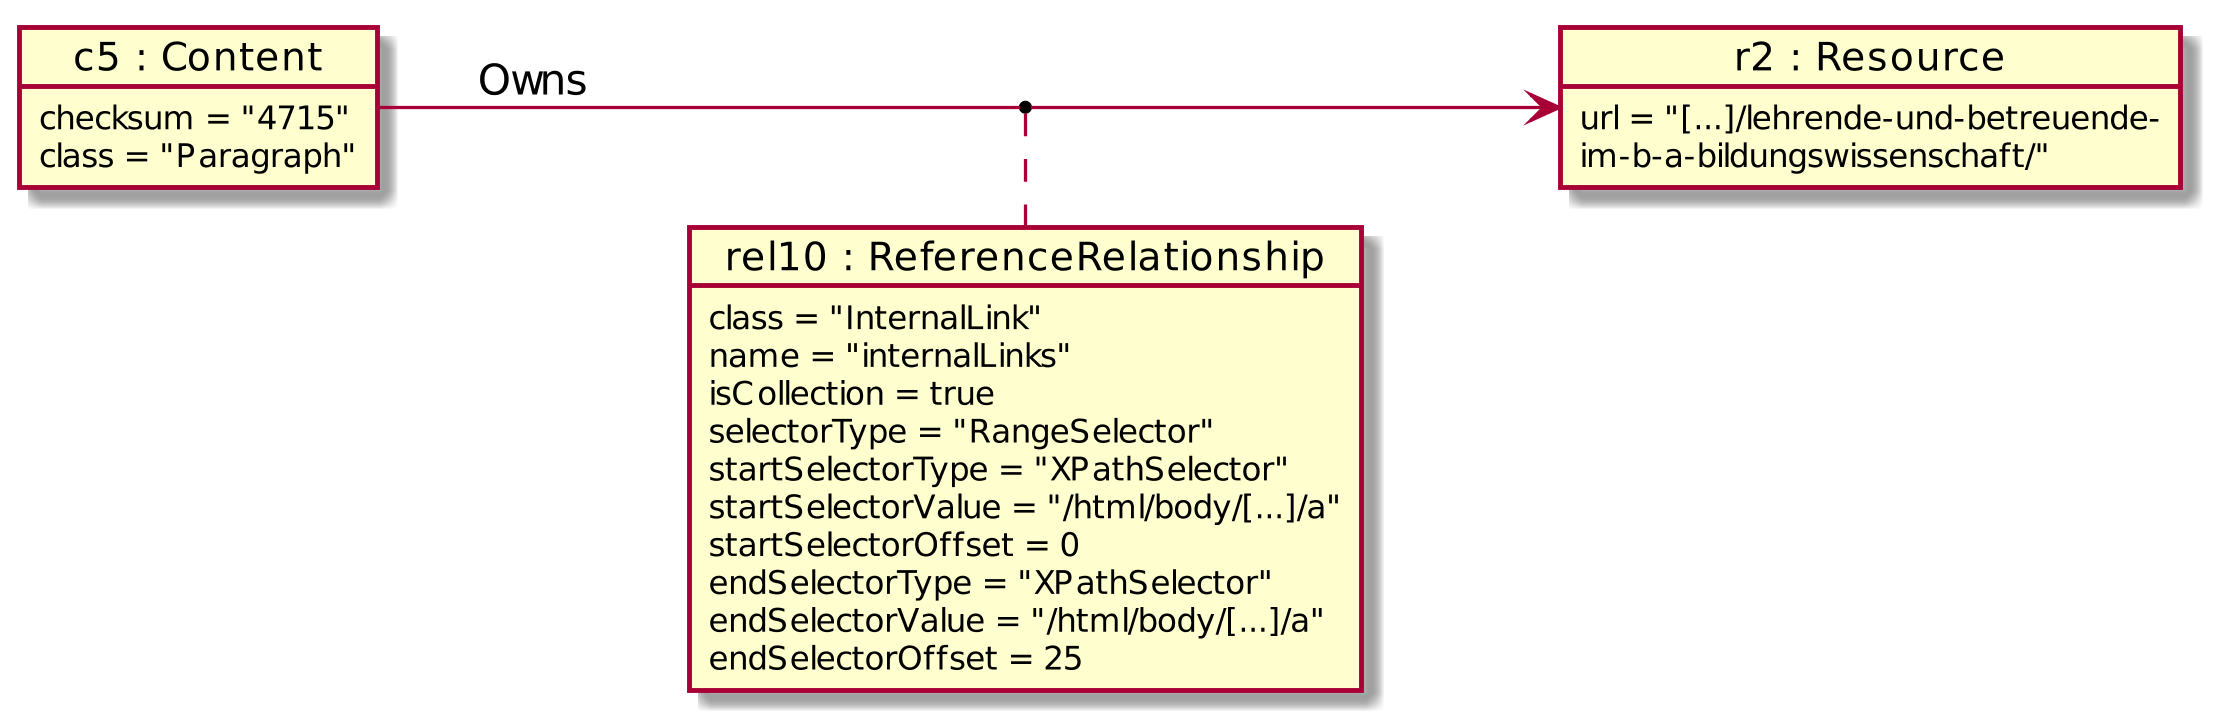
\includegraphics[width=\textwidth]{../resources/db-data-model/example/c5-r2.png}
                \subcaption{Rel 2}                    
            \end{subfigure}
            \caption{Beziehungen}
            \label{image:dbDataModelExampleRelationships}
        \end{figure}

    \subsection{Classification Storage API}
        Wie werden die Daten in die DB geschrieben bzw. gelesen.

    \subsection{Was ist eine Seite}
        \begin{figure}
            \centering
            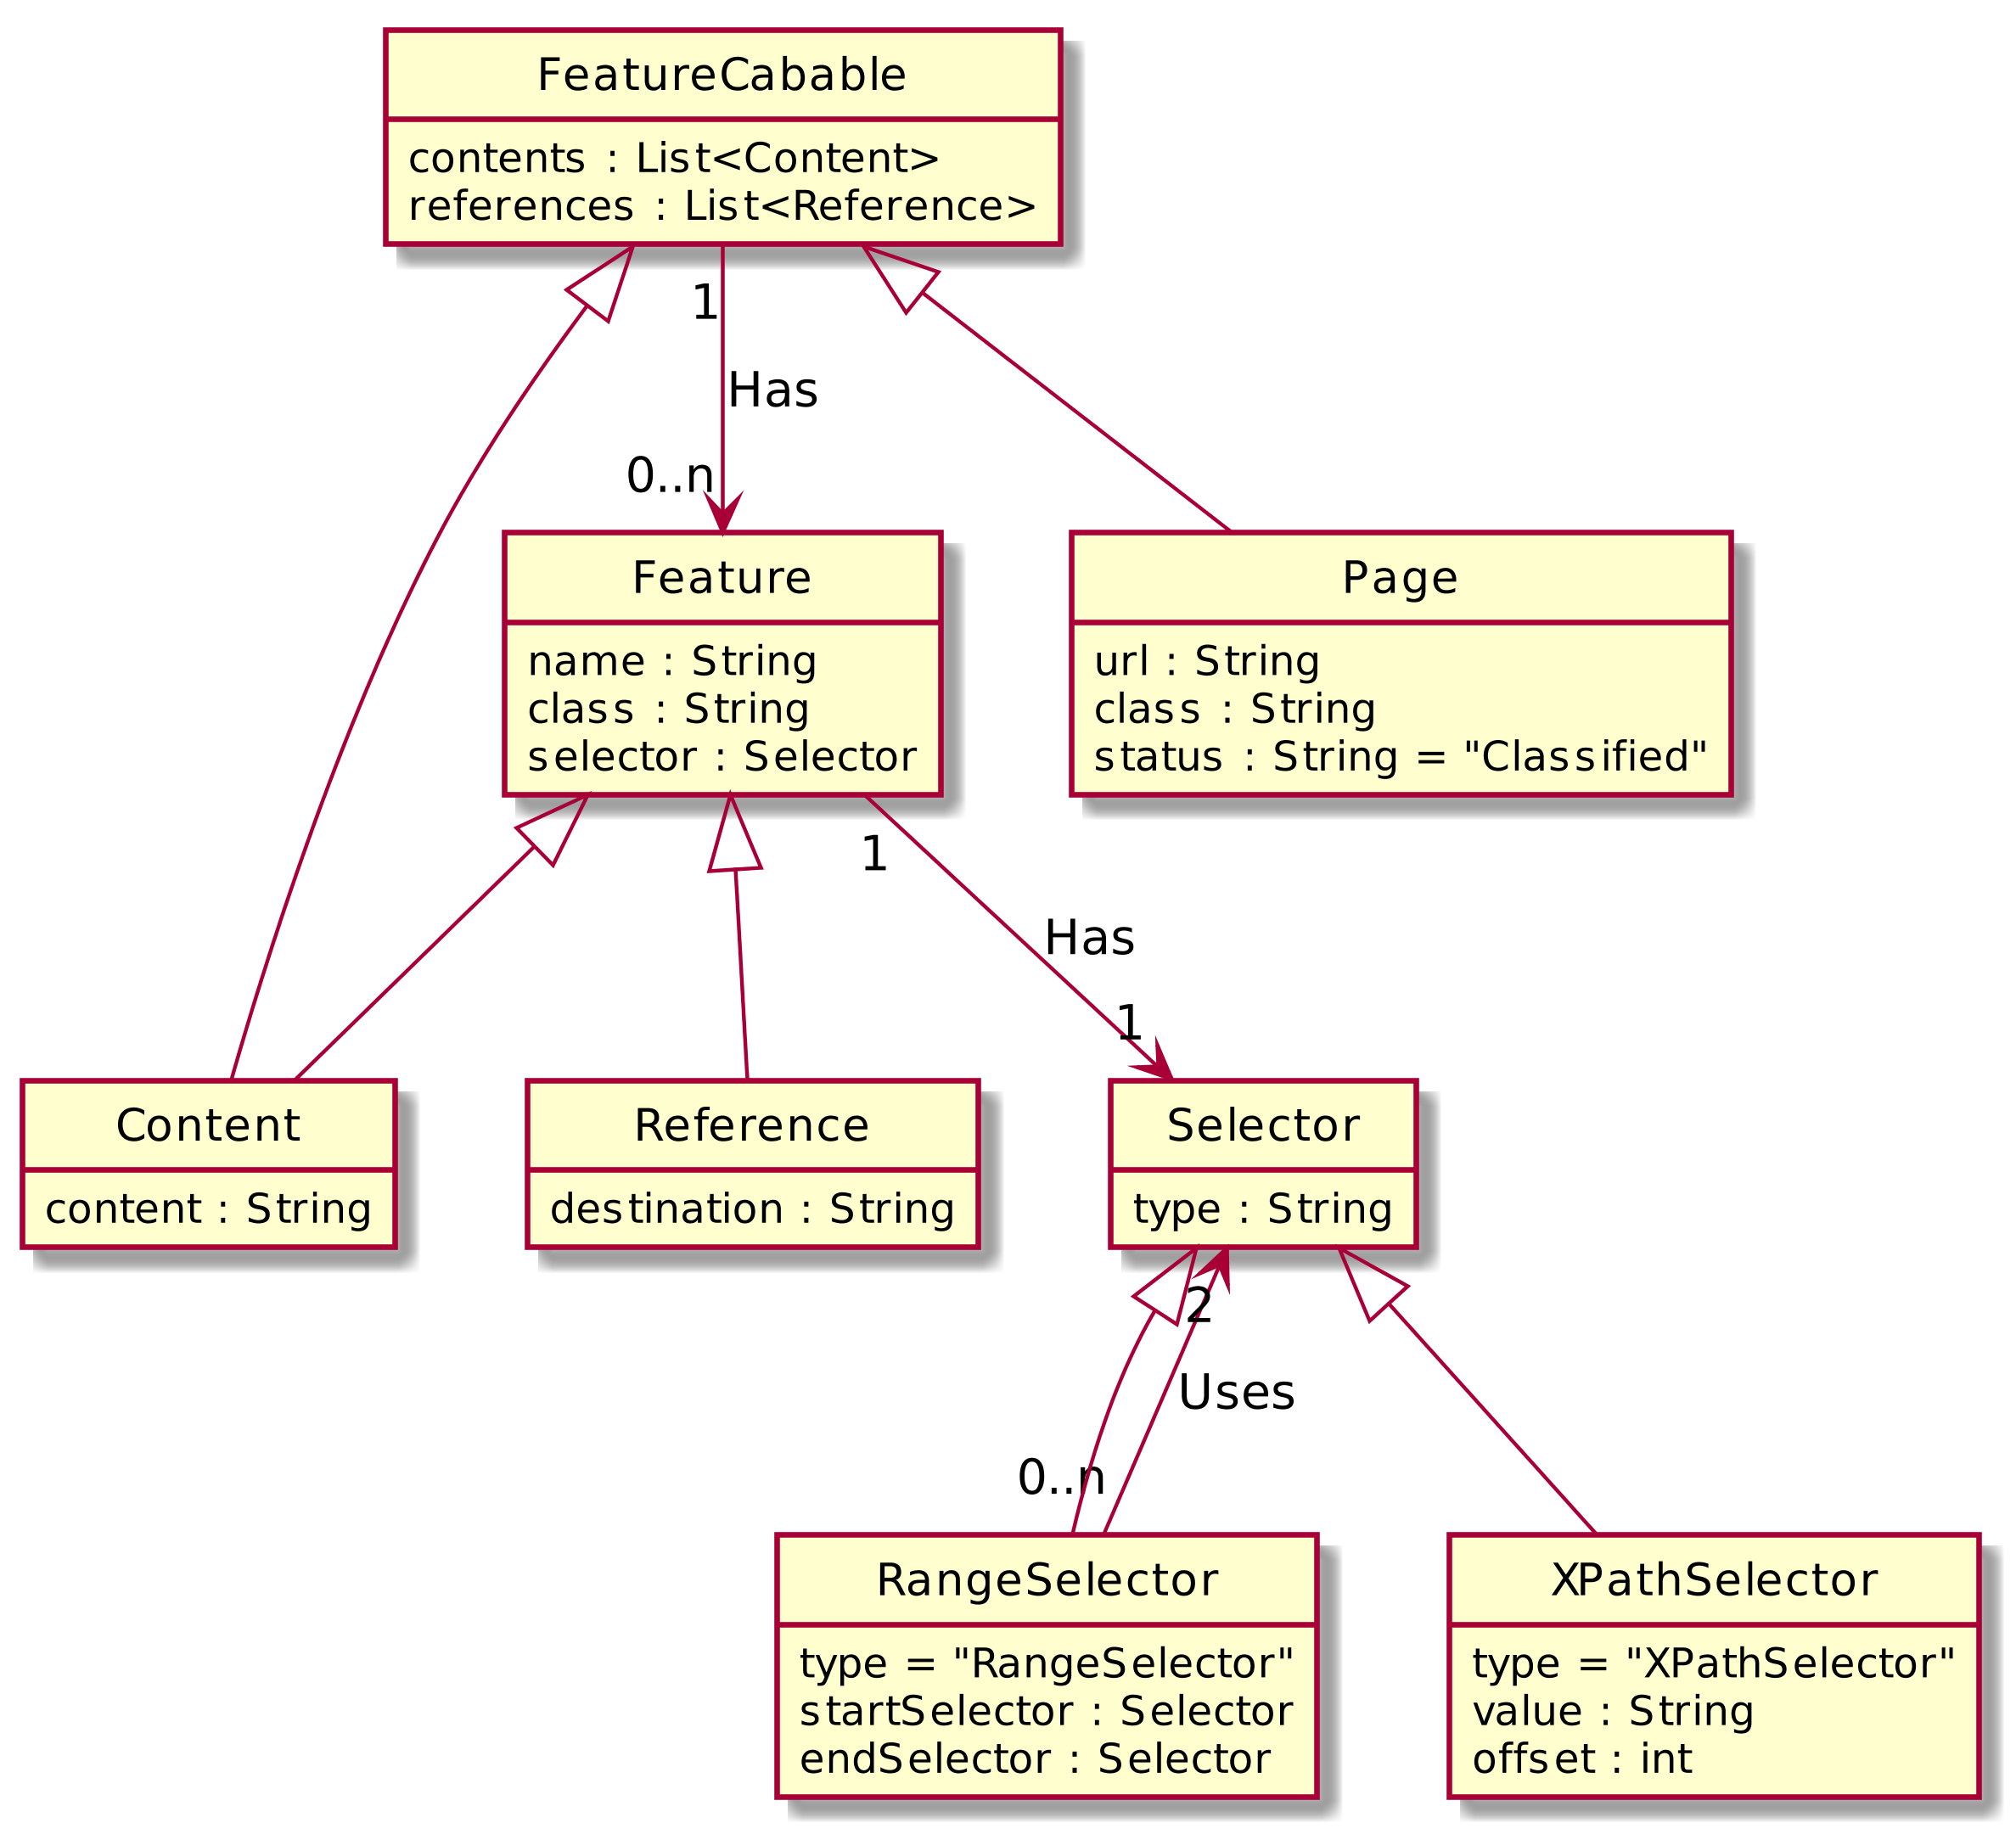
\includegraphics[width=\textwidth]{../resources/storage-api-data-model/page.png}
            \caption{Seite in der Storage API}
            \label{image:storageApiPageModel}
        \end{figure}

    \subsection{Algorithmus zum (initialen) ANLEGEN}
        \lstinputlisting[label=listing:storeClassification,caption=Algorithmus zum Speichern]{../resources/store-classification.code}